\clearpage

\section{Clock\_20171219}

This block doesn't accept any input signal. It outputs one signal that corresponds to a sequence of Dirac's delta functions with a user defined \textit{period}, \textit{phase} and \textit{sampling period}.

\subsection*{Input Parameters}

\begin{itemize}
	\item period\{ 0.0 \};
	\item samplingPeriod\{ 0.0 \};
    \item phase \{0.0\};
\end{itemize}

\subsection*{Methods}

Clock() {}
\bigbreak
Clock(vector$<$Signal *$>$ \&InputSig, vector$<$Signal *$>$ \&OutputSig) :Block(InputSig, OutputSig) {}
\bigbreak
void initialize(void)
\bigbreak
bool runBlock(void)
\bigbreak
void setClockPeriod(double per)
double getClockPeriod()
\bigbreak
void setClockPhase(double pha)
double getClockPhase()
\bigbreak
void setSamplingPeriod(double sPeriod)
double getSamplingPeriod()

\subsection*{Functional description}


\subsection*{Input Signals}

\subparagraph*{Number:} 0

\subsection*{Output Signals}

\subparagraph*{Number:} 1

\subparagraph*{Type:} Sequence of Dirac's delta functions. (TimeContinuousAmplitudeContinuousReal)

\subsection*{Examples}

\begin{figure}[h]
	\centering
	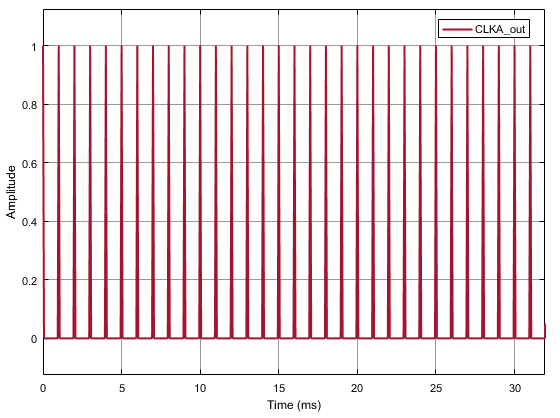
\includegraphics[width=\textwidth]{./lib/clock_20171219/figures/clock_withoutpha}
	\caption{Example of the output signal of the clock without phase shift.}
\end{figure}

\begin{figure}[h]
	\centering
	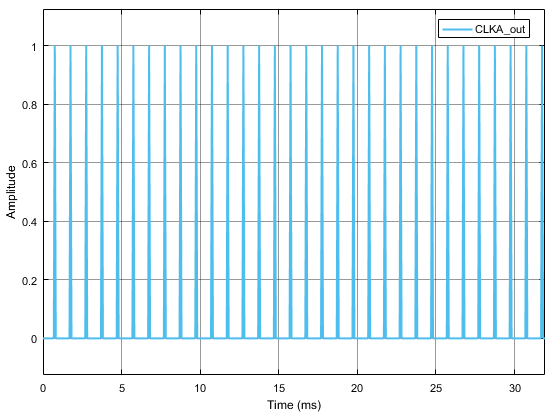
\includegraphics[width=\textwidth]{./lib/clock_20171219/figures/clockPhased}
	\caption{Example of the output signal of the clock with phase shift.}
\end{figure}

\subsection*{Sugestions for future improvement}

